\documentclass[]{thesis-ekf}
\usepackage[T1]{fontenc}
\PassOptionsToPackage{defaults=hu-min}{magyar.ldf}
\usepackage[magyar]{babel}
\usepackage{mathtools,amssymb,amsthm,pdfpages}
\footnotestyle{rule=fourth}

\newtheorem{tetel}{Tétel}[chapter]
\theoremstyle{definition}
\newtheorem{definicio}[tetel]{Definíció}
\theoremstyle{remark}
\newtheorem{megjegyzes}[tetel]{Megjegyzés}

\begin{document}

\institute{Matematikai és Informatikai Intézet}
\title{Színes szkenner megvalósítása egér szenzorral}
\author{Bodnár Máté\\Programtervező informatikus BSc}
\supervisor{Dr. Geda Gábor\\Egyetemi docens}
\city{Eger}
\date{2024}
\maketitle

\tableofcontents

\chapter*{Bevezetés}
\addcontentsline{toc}{chapter}{Bevezetés}


\chapter{Bevezető}

\section{Motiváció}

\section{Célkitűzés}
Egér szenzor általánosságban egy alacsony felbontású monokróm kamera és ebből szines képet akarunk tehát 3 színnel megvilágítva készítünk 3 képet
\chapter{Felhaszánlt technológiák}
\section{Arduino}
\subsection{Arduino platform bemutatása}
forrásként megjelölni a szeegedi egyetemet
\subsection{Az Arduino UNO részei}
A projekt szempontjából megvizsgálni hogy miért ezt választottam
Valamint meg kell nézni a használandó könyvtárakat hogy jók e nanohoz ha váltok
\subsection{Az Arduino alkalmazási területei}
\section{Visual Studio}
\section{Github}
\chapter{Hardveres megvalósítás}
a szenzor mozgatását belevinni
\section{ADNS-9800 szenzor}
\subsection{Működése}
\subsection{Adatok beolvasása}
\section{Adatok továbbítása a Visual Studio felé}
arduino felől rs32 és a studio felé pedig serial
\section{Hardveres bekötés}
smartdraw, circuitikz
\chapter{Szoftveres megvalósítás}
kell mégegy az arduinohoz az arduino szenzor kezelés és szenzor mozgatás
egy alkalmazás amiről tudom kezelni a szkennelést
\section{Beolvasott értékek tárolása 3 dimenzós mátrixban}
adatszeerkezet amiben a beolvasott képet tároljuk
\section{Bikubik interpoláció}
\subsection{Működése}
Működésének alapjai, Matematikai leírása
\section{Mátrix átalakítása képpé}



\chapter*{Összegzés}
Tapasztalatok amiket szereztem a projekt megvalósítása közben
Tovabbfejlesztési gondolatok

színes vagy szürke képet szeretne beolvasni
soros porton küldok egy bitet hogy színes vagy szürke legyen a kép a studiobol
felbontásra vonatkozóan például  feles átfedéssel 
\addcontentsline{toc}{chapter}{Összegzés}

\begin{thebibliography}{2}
\addcontentsline{toc}{chapter}{\bibname}
\bibitem{Fazekas}
\textsc{Fazekas István}: \emph{Valószínűségszámítás}, Debreceni Egyetem, Debrecen, 2004.
\bibitem{Tomacs}
\textsc{Tómács Tibor}: \emph{A valószínűségszámítás alapjai}, Líceum Kiadó, Eger, 2005.
\end{thebibliography}

% Aláírt, szkennelt nyilatkozat beillesztése a szakdolgozat végére
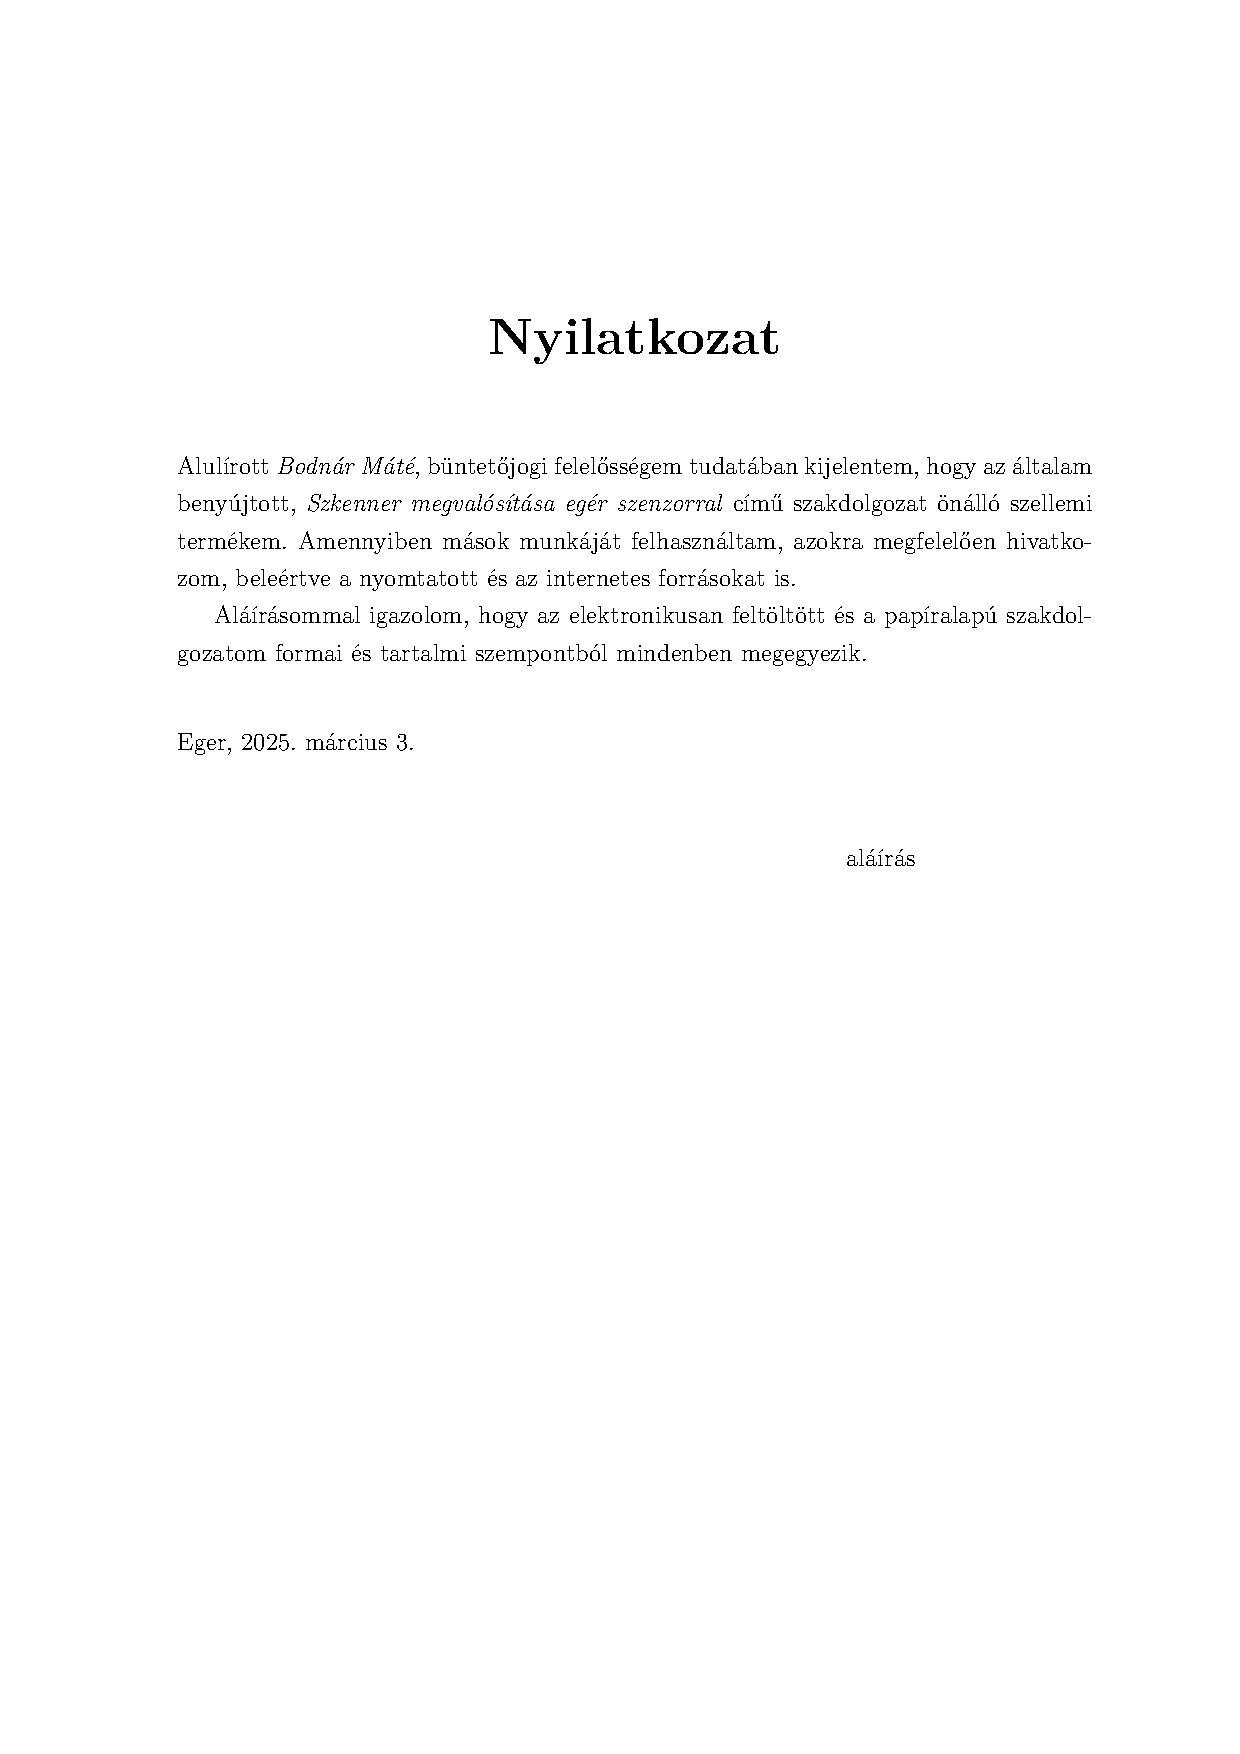
\includepdf{nyilatkozat.pdf}

\end{document}
